\documentclass[aspectratio=169, 10pt]{beamer}
\usetheme{Madrid}
\usefonttheme{professionalfonts}

\usepackage[utf8]{inputenc}
\usepackage[english]{babel}
\usepackage[linguistics]{forest}
\usepackage{algorithmic}
\usepackage{amsfonts}
\usepackage{amsmath}
\usepackage{amssymb}
\usepackage{array}
\usepackage{bookmark}
\usepackage{caption}
\usepackage{colortbl}
\usepackage{csquotes}
\usepackage{graphicx}
\usepackage{hyperref}
\usepackage{lipsum}
\usepackage{lmodern}
\usepackage{mathptmx}
\usepackage{mathtools}
\usepackage{svg}
\usepackage{xcolor}

\hypersetup{
    colorlinks=true,
    linkcolor=blue,
    filecolor=blue,      
    urlcolor=blue,
}

\title{Tutorial 2}
\subtitle{Decision Tree, Cross-validation, Precision and Recall}
\author{Luke Chang}
\institute{The University of Auckland}
\date{Mar. 2021}


\begin{document}

\frame{\titlepage}

%-------------------------------------------------------------------------------
\begin{frame}
\frametitle{Objectives}

\begin{enumerate}
    \item Fully understand Decision Tree and able to explain it in your own words
    \item Compute splitting criterion using Entropy and Information Gain
    \item Fully understand Cross-Validation and know how to use it
    \item Use built-in methods in \texttt{sklearn} to compute ROC and AUC
\end{enumerate}

\end{frame}

%-------------------------------------------------------------------------------
\begin{frame}
\frametitle{Decision Tree Overview}

\begin{itemize}
    \item A decision tree models different possible decision paths, where each decision node is a conditional.
    \item Decision nodes are created based on a \textbf{splitting criterion}.
    \item Most common splitting criterions are: \textbf{Entropy} and \textbf{\href{https://scikit-learn.org/stable/modules/tree.html}{Gini}}.
    \item A tree is created recursively from the root node to the leaf nodes. 
    \item Decision tree can be used for both classification and regression.
\end{itemize}

\end{frame}

%-------------------------------------------------------------------------------
\begin{frame}
\frametitle{Entropy}

Informally, entropy measures the amount of uncertainty in a system.

\begin{block}{Shannon Entropy}
    \[
        H(X) \coloneqq - \sum_x P(X=x) \log_2 P(X=x)
    \]
\end{block}
Where $0 \log_2(0) \equiv 0$, since $\lim_{x \to 0} x \log_2(x)=0$.

\begin{itemize}
    \item<1-> What is the possible maximum entropy?
        \onslide<2->{No upper bound}
    \item<1-> What does it mean?
        \onslide<2->{No better than random guess.}
    \item<1-> What is the possible minimum entropy?
        \onslide<2->{0}
    \item<1-> What does it mean?
        \onslide<2->{You are certain about the outcome. No uncertainty.}
\end{itemize}

\end{frame}

%-------------------------------------------------------------------------------
\begin{frame}{Example: A six-sided Die}
\small
Suppose we have a standard six-sided die with each of the faces has a probability of $1/6$.

\[
    P(X=i) = \frac{1}{6}, i \in \{1,2,3,4,5,6\}
\]

Entropy:

\[
    H(X) = - \sum \frac{1}{6} \log_2 (\frac{1}{6}) = -6[\frac{1}{6} \log_2(\frac{1}{6})] = \log_2(6) \approx 2.6
\]

Suppose we have a loaded six-sided die. All 6 faces are printed ``1''.

\[ P(X=i)= 
    \begin{cases} 
        1 & \text{if } i = 1, \\
        0 & otherwise. 
    \end{cases}
\]

Entropy:

\[
    H(X) = - log_2(1) = 0
\]

\end{frame}

%-------------------------------------------------------------------------------
\begin{frame}
\frametitle{Information Gain}

\begin{block}{Information Gain}
    Information Gain = Parent Entropy - Current Conditional Entropy
    \[
        \text{IG}(Y, X) \coloneqq H(Y) - H(Y|X)
    \]
\end{block}
Where $H(Y|X)$ is the conditional entropy of the target variable $Y$ given attribute $X$ (Weighted sum):

\[
    H(Y|X) \coloneqq \sum_x P(X=x)H(Y|X=x)
\]

And $H(Y|X=x)$ is the conditional entropy of the target variable $Y$ given $X=x$:

\[
    H(Y|X=x) \coloneqq - \sum_y P(Y=y|X=x) \log_2 P(Y=y|X=x)
\]

\end{frame}

%-------------------------------------------------------------------------------
\begin{frame}
\frametitle{Estimating Probabilities}

Let $D_n$ be the subset of the data at node $n$ in the tree, we estimate the probability by counting the number of success:

\[
    P(Y=y) \coloneqq \frac{|\{i \in D_n : i_Y = y\}|}{|D_n|}
\]

Similarly:

\[
    P(X=x) \coloneqq \frac{|\{i \in D_n : i_X = x\}|}{|D_n|}
\]

Conditional probability:

\[
    P(Y=y | X=x) \coloneqq \frac{|\{i \in D_n : i_Y = y \land i_X = x\}|}{|\{i \in D_n : i_X = x \}|}
\]

\end{frame}

%-------------------------------------------------------------------------------
\begin{frame}
\frametitle{Example 1: Boolean Functions}
Give decision trees to represent the following boolean functions:
\begin{enumerate}
    \item $A \land \neg B$
    \item $A \lor (B \land C)$
    \item $A \oplus B$ (XOR)
\end{enumerate}

Question 1: $A \land \neg B$

\begin{table}[]
    \begin{tabular}{lll|l}
    A & B & $\neg$B & Y \\ \hline
    0 & 0 & 1 & 0 \\
    1 & 0 & 1 & 1 \\
    0 & 1 & 0 & 0 \\
    1 & 1 & 0 & 0
    \end{tabular}
\end{table}
    
\end{frame}

%-------------------------------------------------------------------------------
\begin{frame}
\frametitle{$A \land \neg B$ Probabilities}
\small

\begin{columns}
    \begin{column}{0.5\textwidth}
        \begin{table}[]
            \begin{tabular}{lll|l}
            A & B & $\neg$B & Y \\ \hline
            0 & 0 & 1 & 0 \\
            1 & 0 & 1 & 1 \\
            0 & 1 & 0 & 0 \\
            1 & 1 & 0 & 0
            \end{tabular}
        \end{table}
    \end{column}
    \begin{column}{0.5\textwidth}
        \[ P(Y=1) = \frac{1}{4} \]
        % \[ P(A=1) = \frac{2}{4} = \frac{1}{2} \]
        % \[ P(B=1) = \frac{2}{4} = \frac{1}{2} \]
        \[ P(Y=1 | A=1) = \frac{1}{2} \]
        % \[ P(Y=0 | A=1) = \frac{1}{2} \]
        \[ P(Y=1 | A=0) = 0 \]
        % \[ P(Y=0 | A=0) = 1 \]
        \[ P(Y=1 | B=1) = 0 \]
        % \[ P(Y=0 | B=1) = 1 \]
        \[ P(Y=1 | B=0) = \frac{1}{2} \]
        % \[ P(Y=0 | B=0) = \frac{1}{2} \]
    \end{column}
\end{columns}

Root Entropy:
\[
    \begin{split}
        H(Y) & = -P(Y=1) \log_2 P(Y=1) -P(Y=0) \log_2 P(Y=0) \\
                   & = -\frac{1}{4} \log_2(\frac{1}{4}) -\frac{3}{4} \log_2(\frac{3}{4}) \\
                   & \approx 0.5 + 0.31 = 0.81
    \end{split}
\]

\end{frame}

%-------------------------------------------------------------------------------
\begin{frame}
\frametitle{Entropies Condition on A}
\small

\[
    \begin{split}
        H(Y | A=1) & = -P(Y=1 | A=1) \log_2 P(Y=1 | A=1) -P(Y=0 | A=1) \log_2 P(Y=0 | A=1) \\
                   & = -\frac{1}{2} \log_2(\frac{1}{2}) -\frac{1}{2} \log_2(\frac{1}{2}) \\
                   & = 1
    \end{split}
\]

\[
    \begin{split}
        H(Y | A=0) & = -P(Y=1 | A=0) \log_2 P(Y=1 | A=0) -P(Y=0 | A=0) \log_2 P(Y=0 | A=0) \\
                   & = 0
    \end{split}
\]

\[
    \begin{split}
        IG(Y | A) & =  H(Y) - P(A=1)H(Y | A=1) - P(A=0)H(Y | A=0)\\
                  & \approx 0.81 - \frac{2}{4} - 0 = 0.31
    \end{split}
\]

\end{frame}

%-------------------------------------------------------------------------------
\begin{frame}
    \frametitle{Entropies Condition on B}
    \small
    
    \[
        \begin{split}
            H(Y | B=1) & = -P(Y=1 | B=1) \log_2 P(Y=1 | B=1) -P(Y=0 | B=1) \log_2 P(Y=0 | B=1) \\
                       & = 0
        \end{split}
    \]
    
    \[
        \begin{split}
            H(Y | B=0) & = -P(Y=1 | B=0) \log_2 P(Y=1 | B=0) -P(Y=0 | B=0) \log_2 P(Y=0 | B=0) \\
                       & = 1
        \end{split}
    \]
    
    \[
        \begin{split}
            IG(Y | B) & =  H(Y) - P(B=1)H(Y | B=1) - P(B=0)H(Y | B=0)\\
                      & \approx 0.81 - 0 - \frac{2}{4} = 0.31
        \end{split}
    \]
    
\end{frame}

%-------------------------------------------------------------------------------
\begin{frame}
    \frametitle{Information Gain}
    \small
    


    \begin{columns}
        \begin{column}{0.5\textwidth}
            \[
                \begin{split}
                    IG(Y | A) & \approx 0.31\\
                    IG(Y | B) & \approx 0.31\\
                \end{split}
            \]
            
            There is a tie on both conditions. Let's use A as root node.
        \end{column}
        \begin{column}{0.5\textwidth}
            Draw Decision Tree using \texttt{sklearn}
            \begin{figure}
                \centering
                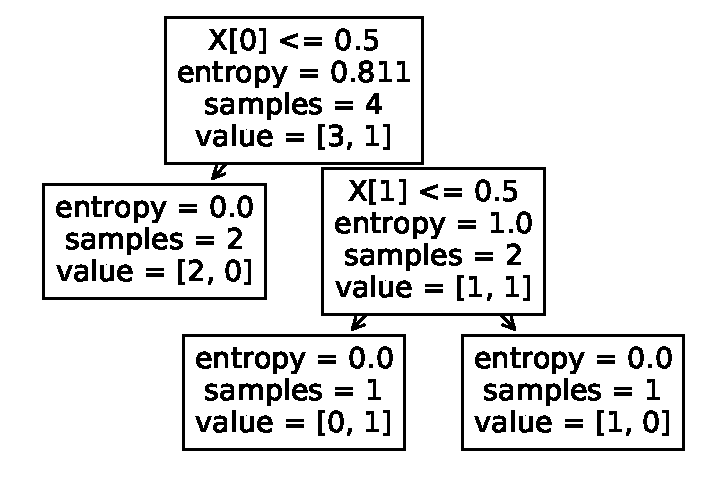
\includegraphics[width=\columnwidth]{../plots/tree_logic_01.pdf}
            \end{figure}
        \end{column}
    \end{columns}

\end{frame}

%-------------------------------------------------------------------------------
\begin{frame}
    \frametitle{Example 2: Questions from last week}
    \small

    \begin{table}[]
        \begin{tabular}{lllll|l}
        Colour & Length & Size & Brightness & Shape & Class \\ \hline
        red & long & larger & bright & triangle & TRUE \\
        red & long & small & bright & circle & FALSE \\
        red & long & small & bright & triangle & TRUE \\
        red & short & larger & dull & circle & FALSE \\
        red & short & larger & bright & triangle & TRUE \\
        blue & short & larger & bright & triangle & FALSE
        \end{tabular}
    \end{table}

    Without prior condition:
    \[
        \begin{split}
            H(Y) & = -P(Y=1) \log_2 P(Y=1) -P(Y=0) \log_2 P(Y=0) \\
                & = -\frac{3}{6} \log_2(\frac{3}{6}) -\frac{3}{6} \log_2(\frac{3}{6}) \\
                & = 0.5 + 0.5 = 1
        \end{split}
    \]

\end{frame}

%-------------------------------------------------------------------------------
\begin{frame}
    \frametitle{Entropies}
    \small

    \begin{table}[]
        \begin{tabular}{lllll|l}
        Colour & Length & Size & Brightness & Shape & Class \\ \hline
        \rowcolor{lightgray} red & long & larger & bright & triangle & \textcolor{red}{TRUE} \\
        \rowcolor{lightgray} red & long & small & bright & circle & FALSE \\
        \rowcolor{lightgray} red & long & small & bright & triangle & \textcolor{red}{TRUE} \\
        \rowcolor{lightgray} red & short & larger & dull & circle & FALSE \\
        \rowcolor{lightgray} red & short & larger & bright & triangle & \textcolor{red}{TRUE} \\
        blue & short & larger & bright & triangle & FALSE
        \end{tabular}
    \end{table}
    
    Condition on \textit{Colour}:
    \[
        \begin{split}
            H(Y|\text{Colour}=\text{red}) & = -\frac{3}{5} log_2(\frac{3}{5}) -\frac{2}{5} log_2(\frac{2}{5}) \approx 0.971 \\
            H(Y|\text{Colour}=\text{blue}) & = 0 \\
            IG(Y|\text{Colour}) & \approx 1 - \frac{5}{6}(0.971) - \frac{1}{6}(0) = 0.191
        \end{split}
    \]
\end{frame}

%-------------------------------------------------------------------------------
\begin{frame}
    \frametitle{Entropies}
    \small

    Condition on \textit{Length}:
    \[
        \begin{split}
            H(Y|\text{Length}=\text{long}) & = -\frac{2}{3} log_2(\frac{2}{3}) -\frac{1}{3} log_2(\frac{1}{3}) \approx 0.918 \\
            H(Y|\text{Length}=\text{short}) & = -\frac{1}{3} log_2(\frac{1}{3}) -\frac{2}{3} log_2(\frac{2}{3}) \approx 0.918 \\
            IG(Y|\text{Length}) & \approx 1 - \frac{3}{6}(0.918) - \frac{3}{6}(0.918) = 0.082
        \end{split}
    \]

    Condition on \textit{Size}:
    \[
        \begin{split}
            H(Y|\text{Size}=\text{large}) & = -\frac{2}{4} log_2(\frac{2}{4}) -\frac{2}{4} log_2(\frac{2}{4}) = 1 \\
            H(Y|\text{Size}=\text{small}) & = -\frac{1}{2} log_2(\frac{1}{2}) -\frac{1}{2} log_2(\frac{1}{2}) = 1 \\
            IG(Y|\text{Size}) & = 1 - \frac{4}{6} - \frac{2}{6} = 0
        \end{split}
    \]

\end{frame}

%-------------------------------------------------------------------------------
\begin{frame}
    \frametitle{Entropies}
    \small

    Condition on \textit{Brightness}:
    \[
        \begin{split}
            H(Y|\text{Brightness}=\text{dull}) & = -\frac{0}{1} log_2(\frac{0}{1}) -\frac{1}{1} log_2(\frac{1}{1}) = 0 \\
            H(Y|\text{Brightness}=\text{bright}) & = -\frac{3}{5} log_2(\frac{3}{5}) -\frac{2}{5} log_2(\frac{2}{5}) \approx 0.971 \\
            IG(Y|\text{Brightness}) & \approx 1 - \frac{1}{6}(0) -\frac{5}{6}(0.971) = 0.191
        \end{split}
    \]

    Condition on \textit{Shape}:
    \[
        \begin{split}
            H(Y|\text{Shape}=\text{triangle}) & = -\frac{3}{4} log_2(\frac{3}{4}) -\frac{1}{4} log_2(\frac{1}{4}) \approx 0.821 \\
            H(Y|\text{Shape}=\text{circle}) & = -\frac{0}{2} log_2(\frac{0}{2}) -\frac{2}{2} log_2(\frac{2}{2}) = 0 \\
            IG(Y|\text{Shape}) & = 1 - \frac{4}{6}(0.821) - \frac{2}{6}(0) = 0.453
        \end{split}
    \]
    
\end{frame}

%-------------------------------------------------------------------------------
\begin{frame}
    \frametitle{Entropies}
    \small
    
    \begin{table}[]
        \begin{tabular}{lr}
            Attribute & Information Gain \\ \hline
            Colour & 0.191 \\
            Length & 0.082 \\
            Size   & 0 \\
            Brightness & 0.191 \\
            Shape & 0.453 \\
        \end{tabular}
    \end{table}

    \textit{Shape} has the largest IG. It is the top of the tree.\\
    \textit{Circle} branch is pure, so it is a leaf. \\
    \textit{triangle} must recurse.

    \begin{center}
        \begin{forest}
            [Shape (Root)[circle (Leaf)][triangle]]
        \end{forest}
    \end{center}

\end{frame}

%-------------------------------------------------------------------------------
\begin{frame}
    \frametitle{Splitting on Shape}
    \small

    \begin{table}[]
        \begin{tabular}{cccccc|l}
        Colour & Length & Size & Brightness & Shape & Class \\ \hline
        \rowcolor{lightgray} red & long & larger & bright & triangle & TRUE \\
        red & long & small & bright & circle & FALSE \\
        \rowcolor{lightgray} red & long & small & bright & triangle & TRUE \\
        red & short & larger & dull & circle & FALSE \\
        \rowcolor{lightgray} red & short & larger & bright & triangle & TRUE \\
        \rowcolor{lightgray} blue & short & larger & bright & triangle & FALSE
        \end{tabular}
    \end{table}

    Given $\text{Shape}=\text{triangle}$, condition on \textit{Colour}:

    \[
        \begin{split}
            H(Y|\text{Shape}=\text{triangle}) & \approx 0.821 \\
            H(Y|\text{Colour}=\text{red}, \text{Shape}=\text{triangle}) & = -\frac{3}{3} log_2(\frac{3}{3}) -\frac{0}{3} log_2(\frac{0}{3}) = 0 \\
            H(Y|\text{Colour}=\text{blue}, \text{Shape}=\text{triangle}) & = -\frac{0}{1} log_2(\frac{0}{1}) -\frac{1}{1} log_2(\frac{1}{1}) = 0 \\
            IG(Y|\text{Colour}, \text{Shape}=\text{triangle}) & \approx \textcolor{orange}{0.821} - 0 - 0 = 0.821
        \end{split}
    \]
\end{frame}

%-------------------------------------------------------------------------------
\begin{frame}
    \frametitle{Splitting on Shape}
    \small
    \[ H(Y|\text{Shape}=\text{triangle}) \approx 0.821 \]

    Given $\text{Shape}=\text{triangle}$, condition on \textit{Length}:

    \[
        \begin{split}
            H(Y|\text{Length}=\text{long}, \text{Shape}=\text{triangle}) & = -\frac{2}{2} log_2(\frac{2}{2}) -\frac{0}{2} log_2(\frac{0}{2}) = 0 \\
            H(Y|\text{Length}=\text{short}, \text{Shape}=\text{triangle}) & = -\frac{1}{2} log_2(\frac{1}{2}) -\frac{1}{2} log_2(\frac{1}{2}) = 1 \\
            IG(Y|\text{Length}, \text{Shape}=\text{triangle}) & \approx \textcolor{orange}{0.821} - 0 - \frac{2}{4} = 0.321
        \end{split}
    \]

    Given $\text{Shape}=\text{triangle}$, condition on \textit{Size}:

    \[
        \begin{split}
            H(Y|\text{Size}=\text{larger}, \text{Shape}=\text{triangle}) & = -\frac{2}{3} log_2(\frac{2}{3}) -\frac{1}{3} log_2(\frac{1}{3}) = 0.918 \\
            H(Y|\text{Size}=\text{small}, \text{Shape}=\text{triangle}) & = -\frac{1}{1} log_2(\frac{1}{1}) -\frac{0}{1} log_2(\frac{0}{1}) = 0 \\
            IG(Y|\text{Size}, \text{Shape}=\text{triangle}) & \approx \textcolor{orange}{0.821} - \frac{3}{4}(0.918) - 0 \approx 0.132
        \end{split}
    \]

\end{frame}

%-------------------------------------------------------------------------------
\begin{frame}
    \frametitle{Splitting on Shape}
    \small
    \[ H(Y|\text{Shape}=\text{triangle}) \approx 0.821 \]

    Given $\text{Shape}=\text{triangle}$, condition on \textit{Brightness}:

    \[
        \begin{split}
            H(Y|\text{Brightness}=\text{dull}, \text{Shape}=\text{triangle}) & = -\frac{3}{4} log_2(\frac{3}{4}) -\frac{1}{4} log_2(\frac{1}{4}) = 0.821 \\
            H(Y|\text{Brightness}=\text{bright}, \text{Shape}=\text{triangle}) & = 0 \\
            IG(Y|\text{Brightness}, \text{Shape}=\text{triangle}) & \approx \textcolor{orange}{0.821} - \frac{4}{4}(0.821) - 0 = 0
        \end{split}
    \]
\end{frame}

%-------------------------------------------------------------------------------
\begin{frame}
    \frametitle{Splitting on Colour}
    \small
    
    \begin{table}[]
        \begin{tabular}{lr}
            Attribute & Information Gain \\ \hline
            Colour & 0.821 \\
            Length & 0.321 \\
            Size   & 0.132 \\
            Brightness & 0 \\
        \end{tabular}
    \end{table}

    The next node is \textit{Colour}.\\
    \textit{Blue} branch is pure and is a leaf. \\
    \textit{Red} branch is pure and is a leaf. \\
    Recursion stops. The entropies of leaf nodes are 0.

    \begin{center}
        \begin{forest}
            [Shape (Root)[circle (Leaf)][triangle[Colour[blue(Leaf)][red(Leaf)]]]]
        \end{forest}
    \end{center}

\end{frame}

%-------------------------------------------------------------------------------
\begin{frame}
    \frametitle{Cross-Validation (CV)}
    
    \begin{itemize}
        \item K-folds Cross-validation uses $k-1$ of the folds as training data.
        \item The performance measure reported by CV is then the average of the values computed in the loop. 
        \item CV should be used only for finding hyper-parameters. 
        \item CV does not shuffle the test set.
        \item Once we obtained the optimal hyper-parameters, we retrain the model with the entire training set.
    \end{itemize}
    
    \begin{figure}
        \centering
        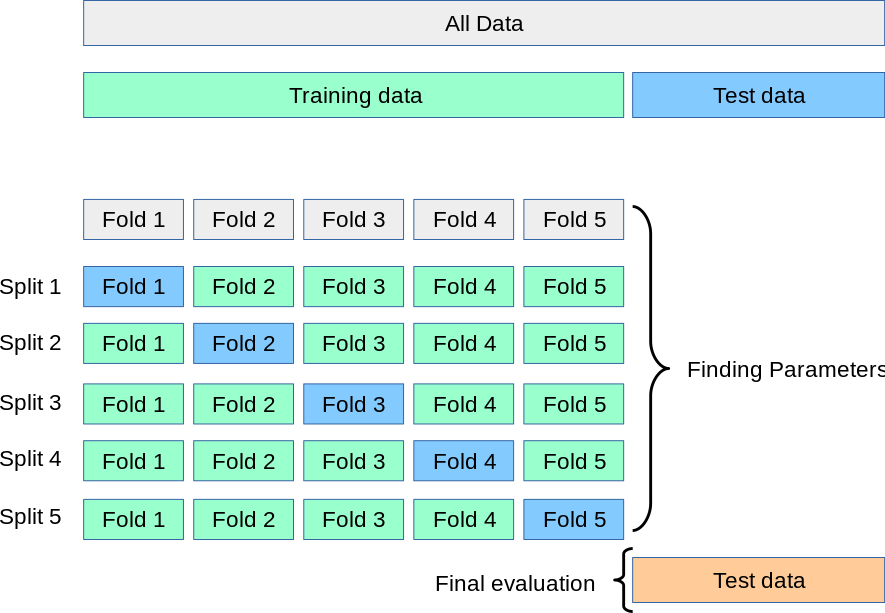
\includegraphics[width=0.45\columnwidth]{../imgs/grid_search_cross_validation.png}
    \end{figure}

\end{frame}

%-------------------------------------------------------------------------------
\begin{frame}
    \frametitle{Code Demos}
    
    Check notebook \texttt{tutorial\_02.ipynb} for code examples.

\end{frame}

\end{document}
